\documentclass[twoside]{book}

% Packages required by doxygen
\usepackage{fixltx2e}
\usepackage{calc}
\usepackage{doxygen}
\usepackage[export]{adjustbox} % also loads graphicx
\usepackage{graphicx}
\usepackage[utf8]{inputenc}
\usepackage{makeidx}
\usepackage{multicol}
\usepackage{multirow}
\PassOptionsToPackage{warn}{textcomp}
\usepackage{textcomp}
\usepackage[nointegrals]{wasysym}
\usepackage[table]{xcolor}

% Font selection
\usepackage[T1]{fontenc}
\usepackage[scaled=.90]{helvet}
\usepackage{courier}
\usepackage{amssymb}
\usepackage{sectsty}
\renewcommand{\familydefault}{\sfdefault}
\allsectionsfont{%
  \fontseries{bc}\selectfont%
  \color{darkgray}%
}
\renewcommand{\DoxyLabelFont}{%
  \fontseries{bc}\selectfont%
  \color{darkgray}%
}
\newcommand{\+}{\discretionary{\mbox{\scriptsize$\hookleftarrow$}}{}{}}

% Page & text layout
\usepackage{geometry}
\geometry{%
  a4paper,%
  top=2.5cm,%
  bottom=2.5cm,%
  left=2.5cm,%
  right=2.5cm%
}
\tolerance=750
\hfuzz=15pt
\hbadness=750
\setlength{\emergencystretch}{15pt}
\setlength{\parindent}{0cm}
\setlength{\parskip}{3ex plus 2ex minus 2ex}
\makeatletter
\renewcommand{\paragraph}{%
  \@startsection{paragraph}{4}{0ex}{-1.0ex}{1.0ex}{%
    \normalfont\normalsize\bfseries\SS@parafont%
  }%
}
\renewcommand{\subparagraph}{%
  \@startsection{subparagraph}{5}{0ex}{-1.0ex}{1.0ex}{%
    \normalfont\normalsize\bfseries\SS@subparafont%
  }%
}
\makeatother

% Headers & footers
\usepackage{fancyhdr}
\pagestyle{fancyplain}
\fancyhead[LE]{\fancyplain{}{\bfseries\thepage}}
\fancyhead[CE]{\fancyplain{}{}}
\fancyhead[RE]{\fancyplain{}{\bfseries\leftmark}}
\fancyhead[LO]{\fancyplain{}{\bfseries\rightmark}}
\fancyhead[CO]{\fancyplain{}{}}
\fancyhead[RO]{\fancyplain{}{\bfseries\thepage}}
\fancyfoot[LE]{\fancyplain{}{}}
\fancyfoot[CE]{\fancyplain{}{}}
\fancyfoot[RE]{\fancyplain{}{\bfseries\scriptsize Generated by Doxygen }}
\fancyfoot[LO]{\fancyplain{}{\bfseries\scriptsize Generated by Doxygen }}
\fancyfoot[CO]{\fancyplain{}{}}
\fancyfoot[RO]{\fancyplain{}{}}
\renewcommand{\footrulewidth}{0.4pt}
\renewcommand{\chaptermark}[1]{%
  \markboth{#1}{}%
}
\renewcommand{\sectionmark}[1]{%
  \markright{\thesection\ #1}%
}

% Indices & bibliography
\usepackage{natbib}
\usepackage[titles]{tocloft}
\setcounter{tocdepth}{3}
\setcounter{secnumdepth}{5}
\makeindex

% Hyperlinks (required, but should be loaded last)
\usepackage{ifpdf}
\ifpdf
  \usepackage[pdftex,pagebackref=true]{hyperref}
\else
  \usepackage[ps2pdf,pagebackref=true]{hyperref}
\fi
\hypersetup{%
  colorlinks=true,%
  linkcolor=blue,%
  citecolor=blue,%
  unicode%
}

% Custom commands
\newcommand{\clearemptydoublepage}{%
  \newpage{\pagestyle{empty}\cleardoublepage}%
}

\usepackage{caption}
\captionsetup{labelsep=space,justification=centering,font={bf},singlelinecheck=off,skip=4pt,position=top}

%===== C O N T E N T S =====

\begin{document}

% Titlepage & ToC
\hypersetup{pageanchor=false,
             bookmarksnumbered=true,
             pdfencoding=unicode
            }
\pagenumbering{alph}
\begin{titlepage}
\vspace*{7cm}
\begin{center}%
{\Large My Project }\\
\vspace*{1cm}
{\large Generated by Doxygen 1.8.12}\\
\end{center}
\end{titlepage}
\clearemptydoublepage
\pagenumbering{roman}
\tableofcontents
\clearemptydoublepage
\pagenumbering{arabic}
\hypersetup{pageanchor=true}

%--- Begin generated contents ---
\chapter{Hierarchical Index}
\section{Class Hierarchy}
This inheritance list is sorted roughly, but not completely, alphabetically\+:\begin{DoxyCompactList}
\item \contentsline{section}{food\+\_\+list}{\pageref{classfood__list}}{}
\item \contentsline{section}{Menu}{\pageref{class_menu}}{}
\item \contentsline{section}{panier}{\pageref{classpanier}}{}
\begin{DoxyCompactList}
\item \contentsline{section}{Panier\+Window}{\pageref{class_panier_window}}{}
\end{DoxyCompactList}
\item \contentsline{section}{plat}{\pageref{classplat}}{}
\begin{DoxyCompactList}
\item \contentsline{section}{boisson}{\pageref{classboisson}}{}
\end{DoxyCompactList}
\item Q\+Dialog\begin{DoxyCompactList}
\item \contentsline{section}{client\+Edit}{\pageref{classclient_edit}}{}
\item \contentsline{section}{Panier\+Window}{\pageref{class_panier_window}}{}
\end{DoxyCompactList}
\item Q\+Main\+Window\begin{DoxyCompactList}
\item \contentsline{section}{Dislike}{\pageref{class_dislike}}{}
\item \contentsline{section}{Home\+Page}{\pageref{class_home_page}}{}
\item \contentsline{section}{Intro\+Window}{\pageref{class_intro_window}}{}
\item \contentsline{section}{Like}{\pageref{class_like}}{}
\item \contentsline{section}{Main\+Window}{\pageref{class_main_window}}{}
\end{DoxyCompactList}
\item Q\+Object\begin{DoxyCompactList}
\item \contentsline{section}{e\+Menu}{\pageref{classe_menu}}{}
\end{DoxyCompactList}
\item Q\+Widget\begin{DoxyCompactList}
\item \contentsline{section}{Client\+Input}{\pageref{class_client_input}}{}
\item \contentsline{section}{plat\+Intro}{\pageref{classplat_intro}}{}
\end{DoxyCompactList}
\end{DoxyCompactList}

\chapter{Class Index}
\section{Class List}
Here are the classes, structs, unions and interfaces with brief descriptions\+:\begin{DoxyCompactList}
\item\contentsline{section}{\hyperlink{classboisson}{boisson} }{\pageref{classboisson}}{}
\item\contentsline{section}{\hyperlink{classclient_edit}{client\+Edit} }{\pageref{classclient_edit}}{}
\item\contentsline{section}{\hyperlink{class_client_input}{Client\+Input} }{\pageref{class_client_input}}{}
\item\contentsline{section}{\hyperlink{class_dislike}{Dislike} }{\pageref{class_dislike}}{}
\item\contentsline{section}{\hyperlink{classe_menu}{e\+Menu} }{\pageref{classe_menu}}{}
\item\contentsline{section}{\hyperlink{classfood__list}{food\+\_\+list} }{\pageref{classfood__list}}{}
\item\contentsline{section}{\hyperlink{class_home_page}{Home\+Page} }{\pageref{class_home_page}}{}
\item\contentsline{section}{\hyperlink{class_intro_window}{Intro\+Window} }{\pageref{class_intro_window}}{}
\item\contentsline{section}{\hyperlink{class_like}{Like} }{\pageref{class_like}}{}
\item\contentsline{section}{\hyperlink{class_main_window}{Main\+Window} }{\pageref{class_main_window}}{}
\item\contentsline{section}{\hyperlink{class_menu}{Menu} }{\pageref{class_menu}}{}
\item\contentsline{section}{\hyperlink{classpanier}{panier} }{\pageref{classpanier}}{}
\item\contentsline{section}{\hyperlink{class_panier_window}{Panier\+Window} }{\pageref{class_panier_window}}{}
\item\contentsline{section}{\hyperlink{classplat}{plat} }{\pageref{classplat}}{}
\item\contentsline{section}{\hyperlink{classplat_intro}{plat\+Intro} }{\pageref{classplat_intro}}{}
\end{DoxyCompactList}

\chapter{Class Documentation}
\hypertarget{classboisson}{}\section{boisson Class Reference}
\label{classboisson}\index{boisson@{boisson}}
Inheritance diagram for boisson\+:\begin{figure}[H]
\begin{center}
\leavevmode
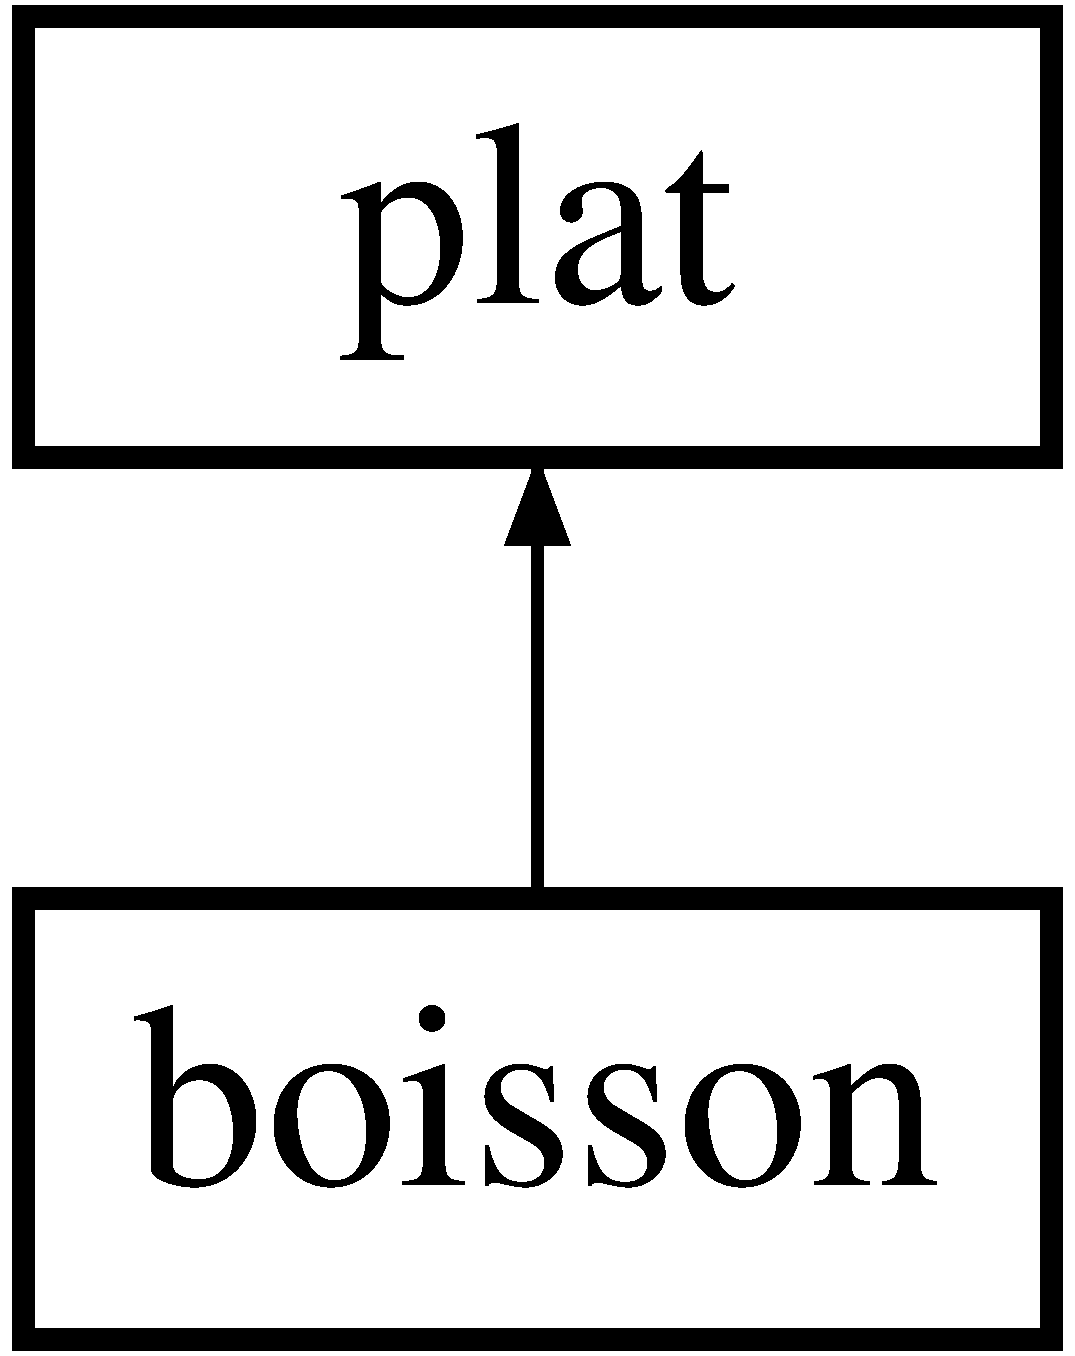
\includegraphics[height=2.000000cm]{classboisson}
\end{center}
\end{figure}
\subsection*{Public Member Functions}
\begin{DoxyCompactItemize}
\item 
{\bfseries boisson} (string \+\_\+nom, int \+\_\+avis=0, int \+\_\+prix=0, const Q\+String \+\_\+image\+Path=\char`\"{}\char`\"{})\hypertarget{classboisson_a9a0fb36038dd58079e657c08c0f24063}{}\label{classboisson_a9a0fb36038dd58079e657c08c0f24063}

\item 
float {\bfseries get\+Alcool\+\_\+degre} () const \hypertarget{classboisson_ad348f3df94927060866925e1e1b1b614}{}\label{classboisson_ad348f3df94927060866925e1e1b1b614}

\item 
void {\bfseries set\+Alcool\+\_\+degre} (float value)\hypertarget{classboisson_abeee81dcdb0f326cd02c841bc8027469}{}\label{classboisson_abeee81dcdb0f326cd02c841bc8027469}

\item 
vector$<$ int $>$ {\bfseries get\+Taille} () const \hypertarget{classboisson_a8d7778f4cf2830b8c504369b3ce15282}{}\label{classboisson_a8d7778f4cf2830b8c504369b3ce15282}

\item 
void {\bfseries set\+Taille} (vector$<$ int $>$ value)\hypertarget{classboisson_a7a7d8042ee2c4c393386df567846eca0}{}\label{classboisson_a7a7d8042ee2c4c393386df567846eca0}

\item 
int {\bfseries get\+Calorie} () const \hypertarget{classboisson_a881251d7b0f9fe313a176400d797bcd3}{}\label{classboisson_a881251d7b0f9fe313a176400d797bcd3}

\item 
void {\bfseries set\+Calorie} (int value)\hypertarget{classboisson_ad56ba9b89833b58895930a590c9ab728}{}\label{classboisson_ad56ba9b89833b58895930a590c9ab728}

\item 
vector$<$ string $>$ {\bfseries get\+Ingredient} () const \hypertarget{classboisson_abe53a0e07c85f529edf06025be68428a}{}\label{classboisson_abe53a0e07c85f529edf06025be68428a}

\item 
void {\bfseries set\+Ingredient} (const vector$<$ string $>$ \&value)\hypertarget{classboisson_afed64ee2018eaf6879297c4470a3b97b}{}\label{classboisson_afed64ee2018eaf6879297c4470a3b97b}

\item 
bool {\bfseries is\+Alcool} ()\hypertarget{classboisson_a42a2dcfb3e56acd9e19b39c575ba06a5}{}\label{classboisson_a42a2dcfb3e56acd9e19b39c575ba06a5}

\item 
void {\bfseries print\+Attrib} ()\hypertarget{classboisson_aad88a1ac4518a46acbc530f5e4b0e9a5}{}\label{classboisson_aad88a1ac4518a46acbc530f5e4b0e9a5}

\end{DoxyCompactItemize}
\subsection*{Additional Inherited Members}


The documentation for this class was generated from the following files\+:\begin{DoxyCompactItemize}
\item 
boisson.\+h\item 
boisson.\+cpp\end{DoxyCompactItemize}

\hypertarget{classclient_edit}{}\section{client\+Edit Class Reference}
\label{classclient_edit}\index{client\+Edit@{client\+Edit}}
Inheritance diagram for client\+Edit\+:\begin{figure}[H]
\begin{center}
\leavevmode
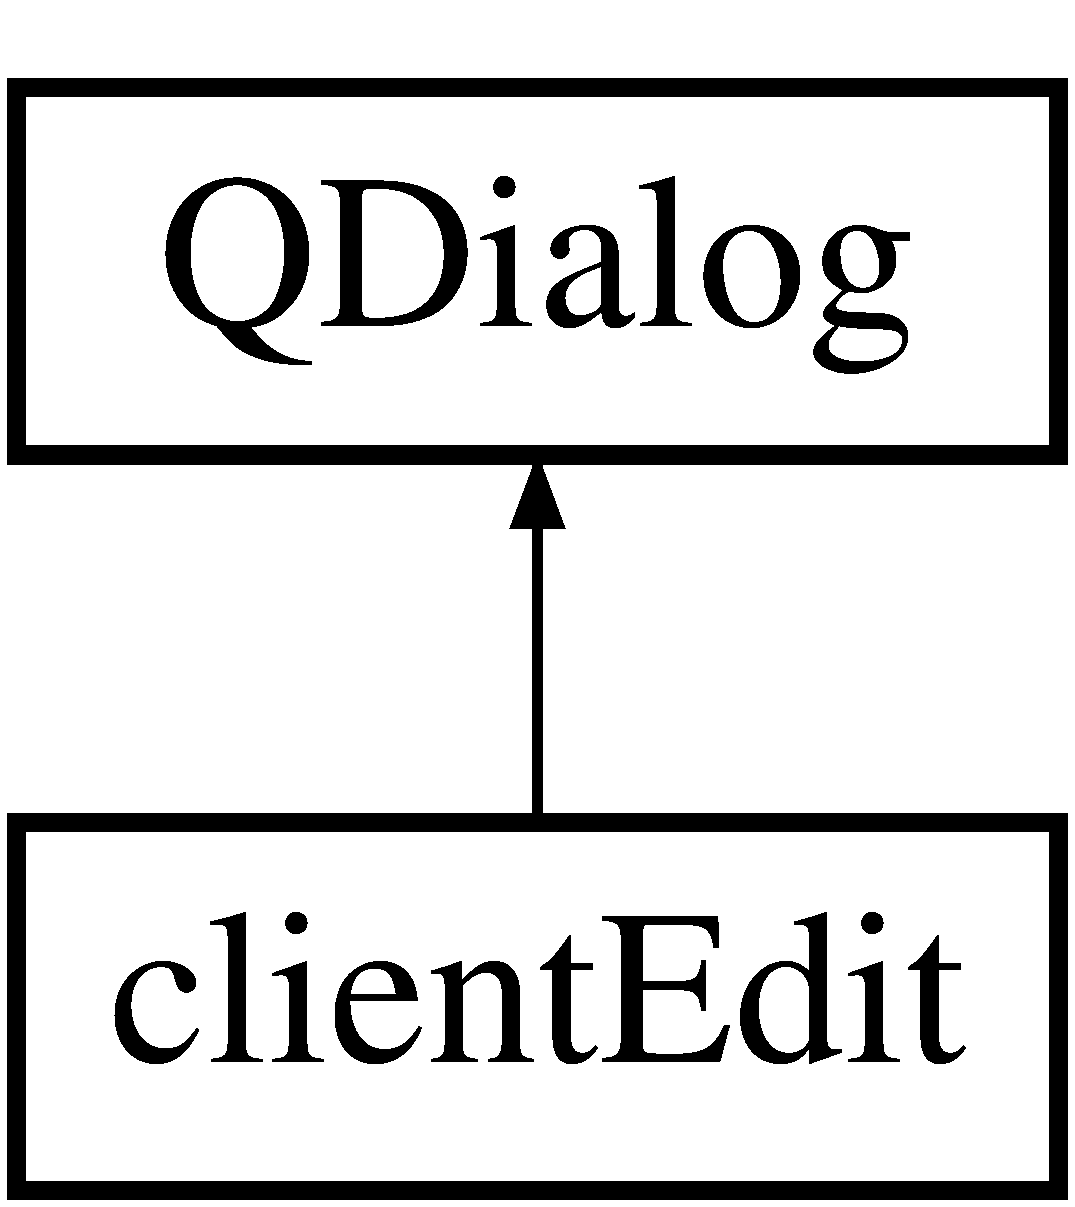
\includegraphics[height=2.000000cm]{classclient_edit}
\end{center}
\end{figure}
\subsection*{Public Slots}
\begin{DoxyCompactItemize}
\item 
void {\bfseries cancel\+Button\+Clicked} ()\hypertarget{classclient_edit_a5a4c7ccbd66ac3e59c0f0d01ea792628}{}\label{classclient_edit_a5a4c7ccbd66ac3e59c0f0d01ea792628}

\item 
void {\bfseries confirm\+Button\+Clicked} ()\hypertarget{classclient_edit_a4e6936dc6537bd38eb13b751fa009b21}{}\label{classclient_edit_a4e6936dc6537bd38eb13b751fa009b21}

\end{DoxyCompactItemize}
\subsection*{Signals}
\begin{DoxyCompactItemize}
\item 
void {\bfseries cancel} (bool)\hypertarget{classclient_edit_afca832860e833415b8f47b1761c388b3}{}\label{classclient_edit_afca832860e833415b8f47b1761c388b3}

\end{DoxyCompactItemize}
\subsection*{Public Member Functions}
\begin{DoxyCompactItemize}
\item 
{\bfseries client\+Edit} (Q\+Widget $\ast$parent=0)\hypertarget{classclient_edit_ac539be9473e6b1525b92393c5dd5c871}{}\label{classclient_edit_ac539be9473e6b1525b92393c5dd5c871}

\end{DoxyCompactItemize}


The documentation for this class was generated from the following files\+:\begin{DoxyCompactItemize}
\item 
clientedit.\+h\item 
clientedit.\+cpp\end{DoxyCompactItemize}

\hypertarget{class_client_input}{}\section{Client\+Input Class Reference}
\label{class_client_input}\index{Client\+Input@{Client\+Input}}
Inheritance diagram for Client\+Input\+:\begin{figure}[H]
\begin{center}
\leavevmode
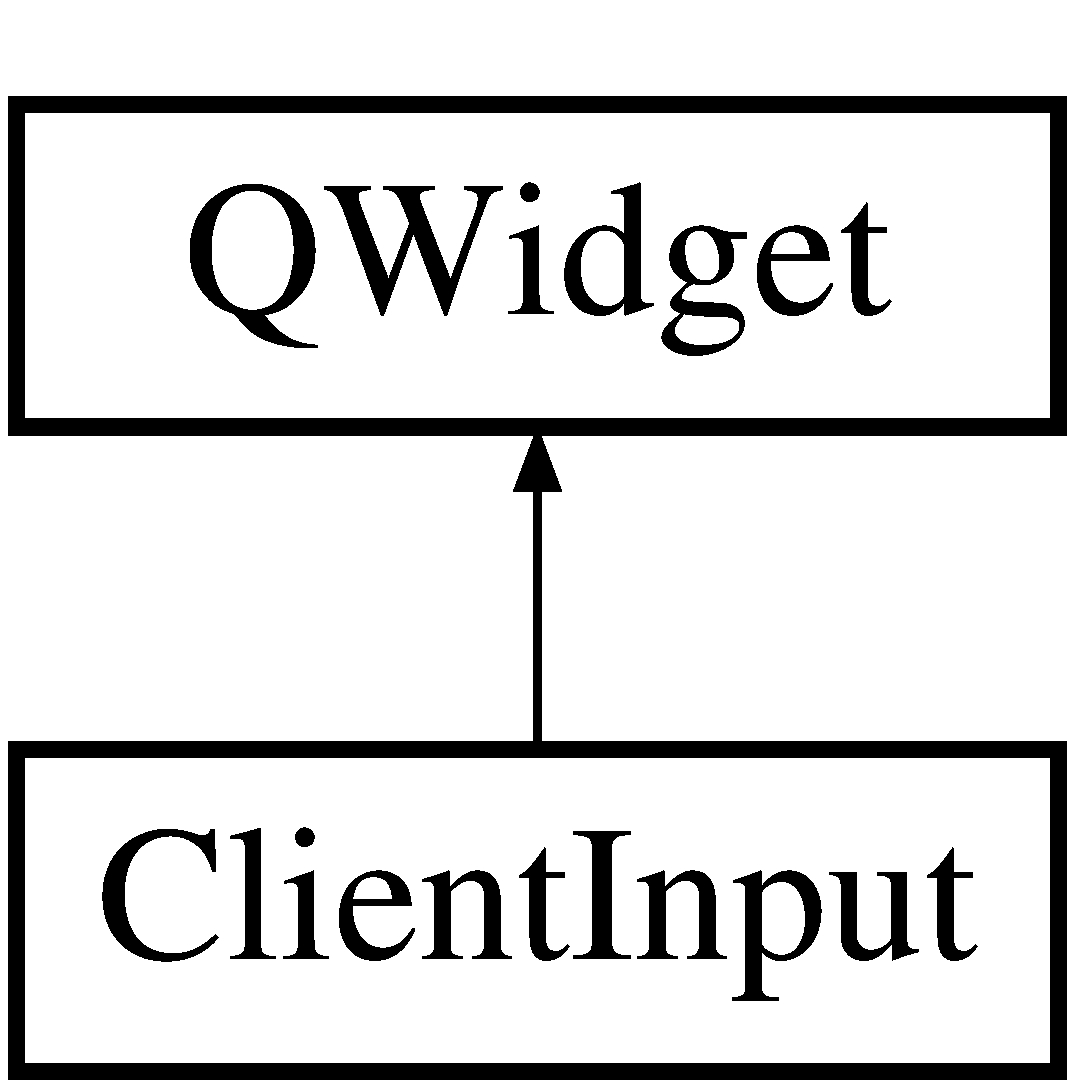
\includegraphics[height=2.000000cm]{class_client_input}
\end{center}
\end{figure}
\subsection*{Public Member Functions}
\begin{DoxyCompactItemize}
\item 
Q\+String {\bfseries get\+Client} (int idx)\hypertarget{class_client_input_aa86836062c0fa1b6518cc5d2c50d3a3b}{}\label{class_client_input_aa86836062c0fa1b6518cc5d2c50d3a3b}

\end{DoxyCompactItemize}
\subsection*{Static Public Member Functions}
\begin{DoxyCompactItemize}
\item 
static \hyperlink{class_client_input}{Client\+Input} \& {\bfseries Instance} ()\hypertarget{class_client_input_aa09466be48687be61c4f64f3648838e5}{}\label{class_client_input_aa09466be48687be61c4f64f3648838e5}

\end{DoxyCompactItemize}


The documentation for this class was generated from the following files\+:\begin{DoxyCompactItemize}
\item 
clientinput.\+h\item 
clientinput.\+cpp\end{DoxyCompactItemize}

\hypertarget{class_dislike}{}\section{Dislike Class Reference}
\label{class_dislike}\index{Dislike@{Dislike}}
Inheritance diagram for Dislike\+:\begin{figure}[H]
\begin{center}
\leavevmode
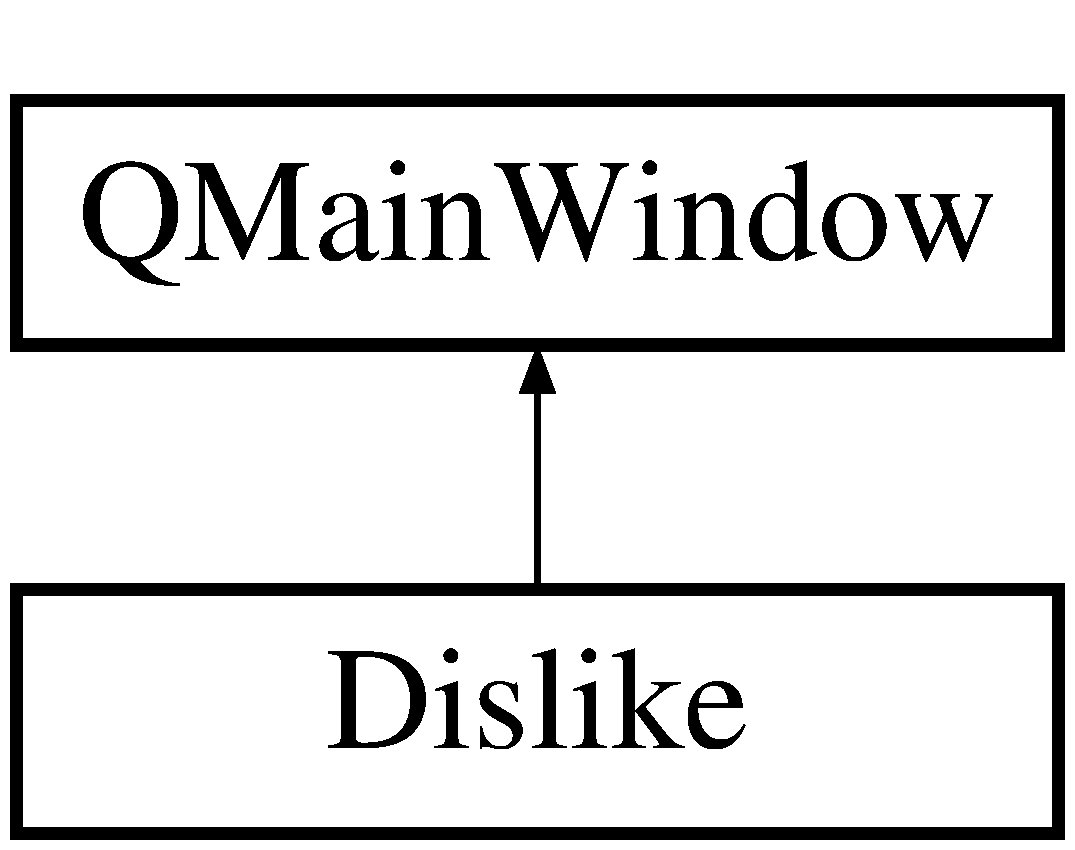
\includegraphics[height=2.000000cm]{class_dislike}
\end{center}
\end{figure}
\subsection*{Public Slots}
\begin{DoxyCompactItemize}
\item 
void {\bfseries confirm\+S\+L\+OT} ()\hypertarget{class_dislike_a16fb4a4bf8f204defa9922e4265b4466}{}\label{class_dislike_a16fb4a4bf8f204defa9922e4265b4466}

\end{DoxyCompactItemize}
\subsection*{Signals}
\begin{DoxyCompactItemize}
\item 
void {\bfseries confirm} ()\hypertarget{class_dislike_a94261e16aa4204d2371c2984366336a7}{}\label{class_dislike_a94261e16aa4204d2371c2984366336a7}

\end{DoxyCompactItemize}
\subsection*{Public Member Functions}
\begin{DoxyCompactItemize}
\item 
{\bfseries Dislike} (Q\+Widget $\ast$parent=0)\hypertarget{class_dislike_aa894589b24751604c1cd4bc0c17422c1}{}\label{class_dislike_aa894589b24751604c1cd4bc0c17422c1}

\item 
Q\+Widget $\ast$ {\bfseries get\+Widget} ()\hypertarget{class_dislike_a342d9eb50e6b382ca8d321517b266375}{}\label{class_dislike_a342d9eb50e6b382ca8d321517b266375}

\end{DoxyCompactItemize}
\subsection*{Public Attributes}
\begin{DoxyCompactItemize}
\item 
int {\bfseries label}\hypertarget{class_dislike_ace5f2fced7fd0b95f322b559af593e99}{}\label{class_dislike_ace5f2fced7fd0b95f322b559af593e99}

\item 
vector$<$ string $>$ {\bfseries ingrediant\+Name}\hypertarget{class_dislike_a2a048ed8ce4e8f050ab229176db58ede}{}\label{class_dislike_a2a048ed8ce4e8f050ab229176db58ede}

\item 
Q\+Check\+Box $\ast$ {\bfseries ing1}\hypertarget{class_dislike_a9a099b3b47a7aa0185348905c49e7eca}{}\label{class_dislike_a9a099b3b47a7aa0185348905c49e7eca}

\item 
Q\+Check\+Box $\ast$ {\bfseries ing2}\hypertarget{class_dislike_a94f61966eedb4ff8d76c90684ea90301}{}\label{class_dislike_a94f61966eedb4ff8d76c90684ea90301}

\item 
Q\+Check\+Box $\ast$ {\bfseries ing3}\hypertarget{class_dislike_aebbb72fcabbd7ca5bc7643b10caf6116}{}\label{class_dislike_aebbb72fcabbd7ca5bc7643b10caf6116}

\item 
Q\+Check\+Box $\ast$ {\bfseries ing4}\hypertarget{class_dislike_a7cc62e686e88d6e1ff9506ed71935b5f}{}\label{class_dislike_a7cc62e686e88d6e1ff9506ed71935b5f}

\item 
Q\+Check\+Box $\ast$ {\bfseries ing5}\hypertarget{class_dislike_afb9c817bcaaa0653cde97568d23497e7}{}\label{class_dislike_afb9c817bcaaa0653cde97568d23497e7}

\item 
Q\+Check\+Box $\ast$ {\bfseries ing6}\hypertarget{class_dislike_a958fddb5800a54a01a9641e776caef9a}{}\label{class_dislike_a958fddb5800a54a01a9641e776caef9a}

\item 
Q\+Check\+Box $\ast$ {\bfseries ing7}\hypertarget{class_dislike_a4aecfa5c8d8b318225481512edd63c97}{}\label{class_dislike_a4aecfa5c8d8b318225481512edd63c97}

\end{DoxyCompactItemize}


The documentation for this class was generated from the following files\+:\begin{DoxyCompactItemize}
\item 
dislike.\+h\item 
dislike.\+cpp\end{DoxyCompactItemize}

\hypertarget{classe_menu}{}\section{e\+Menu Class Reference}
\label{classe_menu}\index{e\+Menu@{e\+Menu}}
Inheritance diagram for e\+Menu\+:\begin{figure}[H]
\begin{center}
\leavevmode
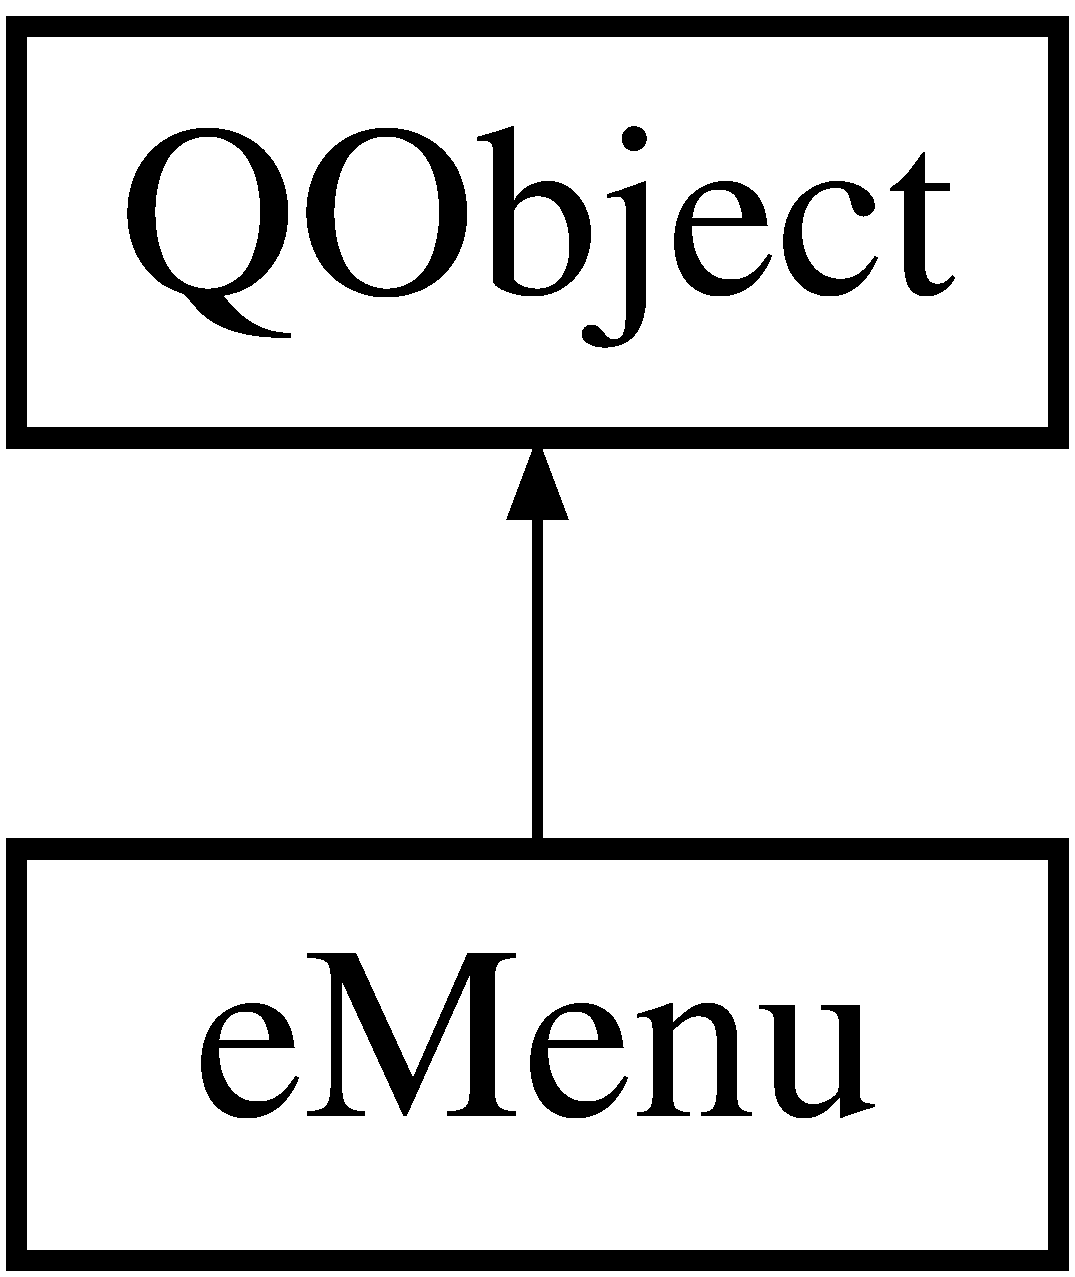
\includegraphics[height=2.000000cm]{classe_menu}
\end{center}
\end{figure}
\subsection*{Public Member Functions}
\begin{DoxyCompactItemize}
\item 
void {\bfseries start} ()\hypertarget{classe_menu_aaf3437a2ac8b478cc955f5baf47edef8}{}\label{classe_menu_aaf3437a2ac8b478cc955f5baf47edef8}

\end{DoxyCompactItemize}


The documentation for this class was generated from the following files\+:\begin{DoxyCompactItemize}
\item 
emenu.\+h\item 
emenu.\+cpp\end{DoxyCompactItemize}

\hypertarget{classfood__list}{}\section{food\+\_\+list Class Reference}
\label{classfood__list}\index{food\+\_\+list@{food\+\_\+list}}
\subsection*{Public Member Functions}
\begin{DoxyCompactItemize}
\item 
{\bfseries food\+\_\+list} (Q\+List\+Widget $\ast$list)\hypertarget{classfood__list_a04af633e55be858e07c281583558ebc8}{}\label{classfood__list_a04af633e55be858e07c281583558ebc8}

\end{DoxyCompactItemize}


The documentation for this class was generated from the following files\+:\begin{DoxyCompactItemize}
\item 
food\+\_\+list.\+h\item 
food\+\_\+list.\+cpp\end{DoxyCompactItemize}

\hypertarget{class_home_page}{}\section{Home\+Page Class Reference}
\label{class_home_page}\index{Home\+Page@{Home\+Page}}
Inheritance diagram for Home\+Page\+:\begin{figure}[H]
\begin{center}
\leavevmode
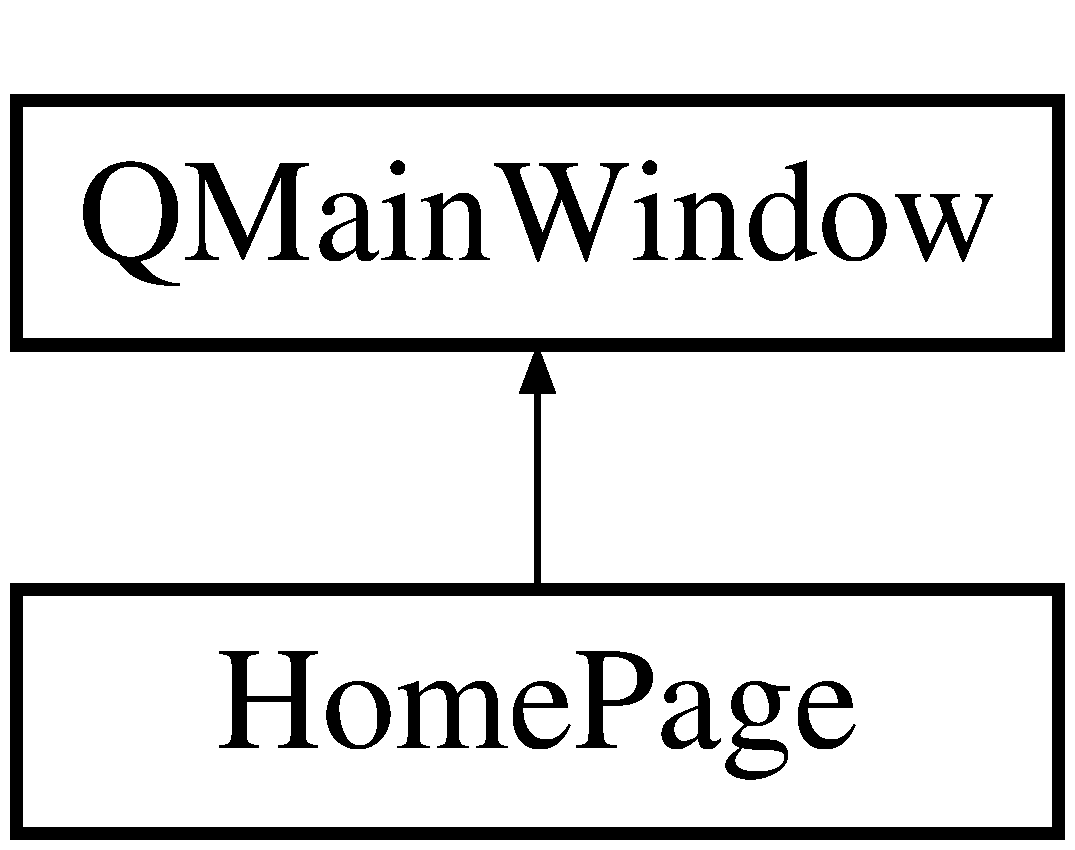
\includegraphics[height=2.000000cm]{class_home_page}
\end{center}
\end{figure}
\subsection*{Public Slots}
\begin{DoxyCompactItemize}
\item 
void {\bfseries menu\+Clicked} ()\hypertarget{class_home_page_abc8305a0e8d66845d6a1c05d91392de0}{}\label{class_home_page_abc8305a0e8d66845d6a1c05d91392de0}

\item 
void {\bfseries order\+Clicked} ()\hypertarget{class_home_page_a09666cd4c6c0bb7b55949f75e9622b7b}{}\label{class_home_page_a09666cd4c6c0bb7b55949f75e9622b7b}

\item 
void {\bfseries help\+Clicked} ()\hypertarget{class_home_page_a91dc194a54ecd1cb111f11d3ada24bec}{}\label{class_home_page_a91dc194a54ecd1cb111f11d3ada24bec}

\end{DoxyCompactItemize}
\subsection*{Signals}
\begin{DoxyCompactItemize}
\item 
void {\bfseries menu} ()\hypertarget{class_home_page_a5c7e38aa4e8ca1385adf4cb6a8a8b3d4}{}\label{class_home_page_a5c7e38aa4e8ca1385adf4cb6a8a8b3d4}

\item 
void {\bfseries order} ()\hypertarget{class_home_page_ac889b971aa6c77c149e92b51525041b2}{}\label{class_home_page_ac889b971aa6c77c149e92b51525041b2}

\item 
void {\bfseries help} ()\hypertarget{class_home_page_a4a759ea4aba519af70052055fa26a12c}{}\label{class_home_page_a4a759ea4aba519af70052055fa26a12c}

\end{DoxyCompactItemize}
\subsection*{Public Member Functions}
\begin{DoxyCompactItemize}
\item 
{\bfseries Home\+Page} (Q\+Widget $\ast$parent=0)\hypertarget{class_home_page_a11aaf93fd8a54885cf046c23501a07aa}{}\label{class_home_page_a11aaf93fd8a54885cf046c23501a07aa}

\end{DoxyCompactItemize}


The documentation for this class was generated from the following files\+:\begin{DoxyCompactItemize}
\item 
homepage.\+h\item 
homepage.\+cpp\end{DoxyCompactItemize}

\hypertarget{class_intro_window}{}\section{Intro\+Window Class Reference}
\label{class_intro_window}\index{Intro\+Window@{Intro\+Window}}
Inheritance diagram for Intro\+Window\+:\begin{figure}[H]
\begin{center}
\leavevmode
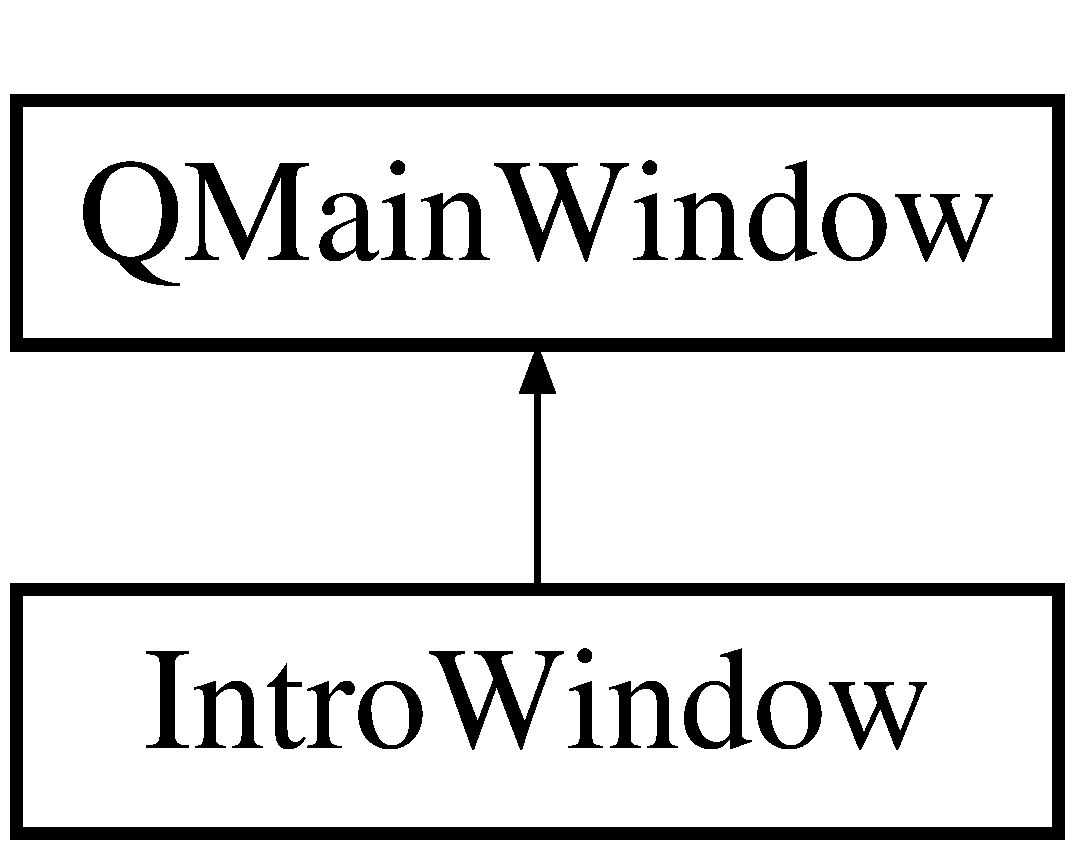
\includegraphics[height=2.000000cm]{class_intro_window}
\end{center}
\end{figure}
\subsection*{Public Slots}
\begin{DoxyCompactItemize}
\item 
void {\bfseries on\+Next\+Clicked} ()\hypertarget{class_intro_window_ab8d051369152d97e08d9dd02635ab999}{}\label{class_intro_window_ab8d051369152d97e08d9dd02635ab999}

\item 
void {\bfseries on\+Skip\+Clicked} ()\hypertarget{class_intro_window_ada6c1a6322bb235d82a7228ffcdc14c0}{}\label{class_intro_window_ada6c1a6322bb235d82a7228ffcdc14c0}

\end{DoxyCompactItemize}
\subsection*{Signals}
\begin{DoxyCompactItemize}
\item 
void {\bfseries F\+I\+N\+I\+S\+H\+ED} ()\hypertarget{class_intro_window_ac7a08d8893736c443e49b80375983e0a}{}\label{class_intro_window_ac7a08d8893736c443e49b80375983e0a}

\end{DoxyCompactItemize}
\subsection*{Public Member Functions}
\begin{DoxyCompactItemize}
\item 
{\bfseries Intro\+Window} (Q\+Widget $\ast$like, Q\+Widget $\ast$\+\_\+dislike, Q\+Widget $\ast$parent=0)\hypertarget{class_intro_window_a20c9761c81730a9548bc3b3ad3d0f602}{}\label{class_intro_window_a20c9761c81730a9548bc3b3ad3d0f602}

\end{DoxyCompactItemize}


The documentation for this class was generated from the following files\+:\begin{DoxyCompactItemize}
\item 
introwindow.\+h\item 
introwindow.\+cpp\end{DoxyCompactItemize}

\hypertarget{class_like}{}\section{Like Class Reference}
\label{class_like}\index{Like@{Like}}
Inheritance diagram for Like\+:\begin{figure}[H]
\begin{center}
\leavevmode
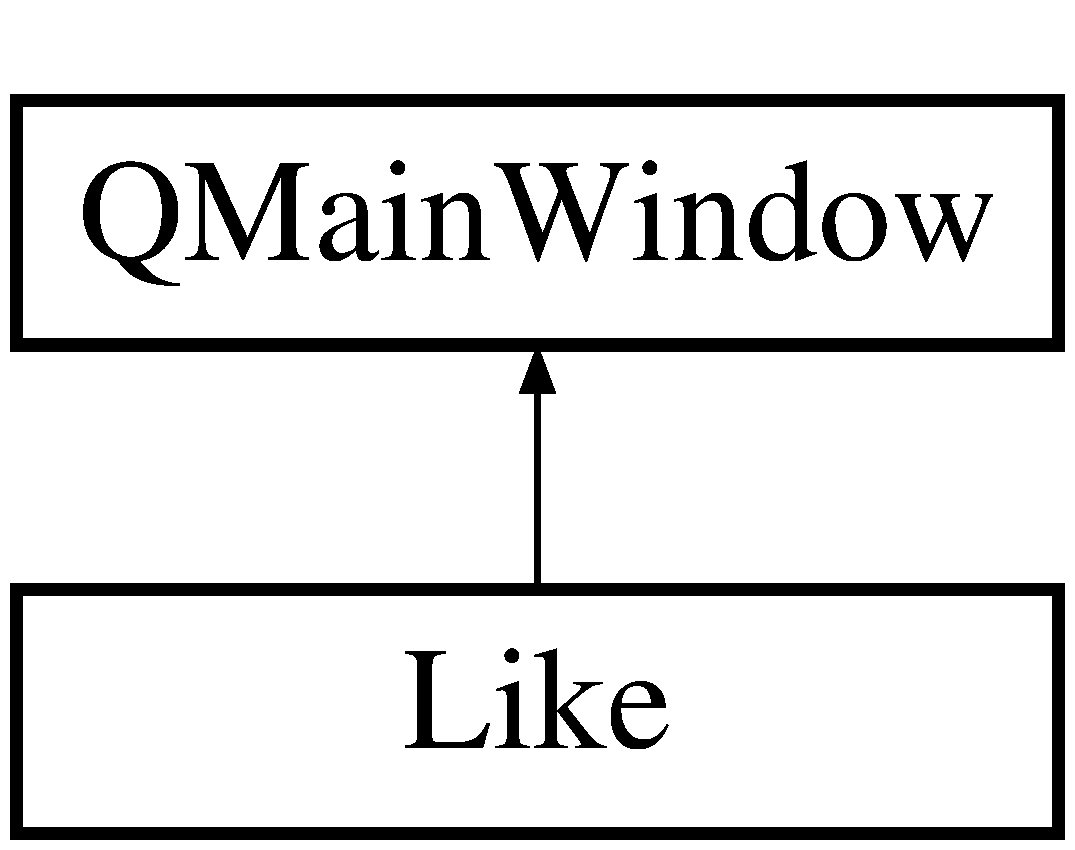
\includegraphics[height=2.000000cm]{class_like}
\end{center}
\end{figure}
\subsection*{Public Slots}
\begin{DoxyCompactItemize}
\item 
void {\bfseries confirm\+S\+L\+OT} ()\hypertarget{class_like_ac5d54e3f22e4ca359c796bb8b3ee02de}{}\label{class_like_ac5d54e3f22e4ca359c796bb8b3ee02de}

\end{DoxyCompactItemize}
\subsection*{Signals}
\begin{DoxyCompactItemize}
\item 
void {\bfseries confirm} ()\hypertarget{class_like_a9c2b32bf16e5a26749783bc24c99d402}{}\label{class_like_a9c2b32bf16e5a26749783bc24c99d402}

\end{DoxyCompactItemize}
\subsection*{Public Member Functions}
\begin{DoxyCompactItemize}
\item 
{\bfseries Like} (Q\+Widget $\ast$parent=0)\hypertarget{class_like_a1e6dca63e0a3c7b7b1fdcf4b4d832167}{}\label{class_like_a1e6dca63e0a3c7b7b1fdcf4b4d832167}

\item 
Q\+Widget $\ast$ {\bfseries get\+Widget} ()\hypertarget{class_like_a502d5988becfb7b16b28a6c2966e8a63}{}\label{class_like_a502d5988becfb7b16b28a6c2966e8a63}

\end{DoxyCompactItemize}
\subsection*{Public Attributes}
\begin{DoxyCompactItemize}
\item 
Q\+Check\+Box $\ast$ {\bfseries ing1}\hypertarget{class_like_a8080eecf6250ec5852f436b9641f3c09}{}\label{class_like_a8080eecf6250ec5852f436b9641f3c09}

\item 
Q\+Check\+Box $\ast$ {\bfseries ing2}\hypertarget{class_like_ad09dec9a7ebc761378e532875bfa31fd}{}\label{class_like_ad09dec9a7ebc761378e532875bfa31fd}

\item 
Q\+Check\+Box $\ast$ {\bfseries ing3}\hypertarget{class_like_a32e570488089a0f2a92689a8f152b334}{}\label{class_like_a32e570488089a0f2a92689a8f152b334}

\item 
Q\+Check\+Box $\ast$ {\bfseries ing4}\hypertarget{class_like_a02ccb8c023f736b7a535cd93eab7612d}{}\label{class_like_a02ccb8c023f736b7a535cd93eab7612d}

\item 
Q\+Check\+Box $\ast$ {\bfseries ing5}\hypertarget{class_like_a08638a9956051cd61102e92e749c7bce}{}\label{class_like_a08638a9956051cd61102e92e749c7bce}

\item 
Q\+V\+Box\+Layout $\ast$ {\bfseries plat\+Layout}\hypertarget{class_like_aacff3597e99f7ab6b31953a5e7103133}{}\label{class_like_aacff3597e99f7ab6b31953a5e7103133}

\item 
int {\bfseries label}\hypertarget{class_like_aa67d5bf4c7d3272671012e2cb4a0e822}{}\label{class_like_aa67d5bf4c7d3272671012e2cb4a0e822}

\item 
vector$<$ string $>$ {\bfseries ingrediant\+Name}\hypertarget{class_like_afa5837420ab339db4ba713e97acac863}{}\label{class_like_afa5837420ab339db4ba713e97acac863}

\item 
vector$<$ \hyperlink{classplat_intro}{plat\+Intro} $\ast$ $>$ {\bfseries list}\hypertarget{class_like_a1852fe305012c8a4a13fdc4cd04dd0b4}{}\label{class_like_a1852fe305012c8a4a13fdc4cd04dd0b4}

\item 
vector$<$ \hyperlink{classplat_intro}{plat\+Intro} $\ast$ $>$ {\bfseries deletedlist}\hypertarget{class_like_a9146ca347e7e59e3eb662ad71ed3f6b8}{}\label{class_like_a9146ca347e7e59e3eb662ad71ed3f6b8}

\end{DoxyCompactItemize}


The documentation for this class was generated from the following files\+:\begin{DoxyCompactItemize}
\item 
like.\+h\item 
like.\+cpp\end{DoxyCompactItemize}

\hypertarget{class_main_window}{}\section{Main\+Window Class Reference}
\label{class_main_window}\index{Main\+Window@{Main\+Window}}
Inheritance diagram for Main\+Window\+:\begin{figure}[H]
\begin{center}
\leavevmode
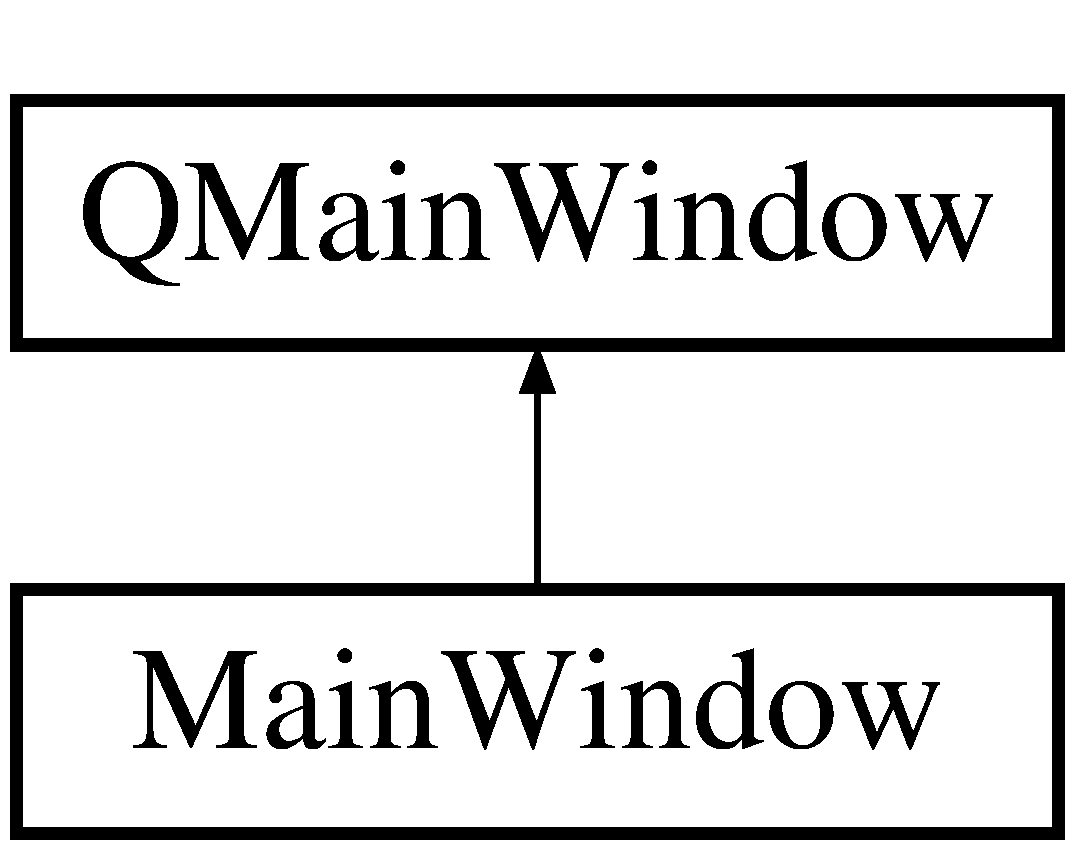
\includegraphics[height=2.000000cm]{class_main_window}
\end{center}
\end{figure}
\subsection*{Signals}
\begin{DoxyCompactItemize}
\item 
void {\bfseries order\+Submitted} ()\hypertarget{class_main_window_a0bf3c8978269c0dc28ad5c86e1364702}{}\label{class_main_window_a0bf3c8978269c0dc28ad5c86e1364702}

\end{DoxyCompactItemize}
\subsection*{Public Member Functions}
\begin{DoxyCompactItemize}
\item 
{\bfseries Main\+Window} (Q\+Widget $\ast$parent=0)\hypertarget{class_main_window_a8b244be8b7b7db1b08de2a2acb9409db}{}\label{class_main_window_a8b244be8b7b7db1b08de2a2acb9409db}

\item 
void {\bfseries update\+Like} (Q\+V\+Box\+Layout $\ast$layout\+\_\+, vector$<$ \hyperlink{classplat_intro}{plat\+Intro} $\ast$ $>$ \&list\+\_\+)\hypertarget{class_main_window_a9ad74def483045acb64534c0f397adbc}{}\label{class_main_window_a9ad74def483045acb64534c0f397adbc}

\item 
void {\bfseries updatedis\+Like} (Q\+V\+Box\+Layout $\ast$layout\+\_\+, vector$<$ \hyperlink{classplat_intro}{plat\+Intro} $\ast$ $>$ \&list\+\_\+)\hypertarget{class_main_window_ae7f2b02aaad962833cd4a5870d50bf07}{}\label{class_main_window_ae7f2b02aaad962833cd4a5870d50bf07}

\item 
void {\bfseries update\+Like} ()\hypertarget{class_main_window_abc427e82a2f09332245c8881cb41625c}{}\label{class_main_window_abc427e82a2f09332245c8881cb41625c}

\item 
void {\bfseries update\+Dislike} ()\hypertarget{class_main_window_a5e2496f25f7b70d6af56fb40ac08487b}{}\label{class_main_window_a5e2496f25f7b70d6af56fb40ac08487b}

\item 
void {\bfseries set\+Client} ()\hypertarget{class_main_window_a62c5fc1c8d38d29783d817704ae529ae}{}\label{class_main_window_a62c5fc1c8d38d29783d817704ae529ae}

\item 
void {\bfseries set\+Preference} (\hyperlink{class_like}{Like} $\ast$\+\_\+like)\hypertarget{class_main_window_af96e41539c9bfd54a30b14ee4cfa7b1e}{}\label{class_main_window_af96e41539c9bfd54a30b14ee4cfa7b1e}

\item 
void {\bfseries set\+Dislike} (\hyperlink{class_dislike}{Dislike} $\ast$\+\_\+dislike)\hypertarget{class_main_window_a5d03cd61b08a4c7954391cb42f2a301c}{}\label{class_main_window_a5d03cd61b08a4c7954391cb42f2a301c}

\end{DoxyCompactItemize}
\subsection*{Public Attributes}
\begin{DoxyCompactItemize}
\item 
vector$<$ \hyperlink{classplat_intro}{plat\+Intro} $\ast$ $>$ {\bfseries entree\+List}\hypertarget{class_main_window_a3f7f02da1ccf53028290322b93fa42e2}{}\label{class_main_window_a3f7f02da1ccf53028290322b93fa42e2}

\item 
vector$<$ \hyperlink{classplat_intro}{plat\+Intro} $\ast$ $>$ {\bfseries plat\+List}\hypertarget{class_main_window_a4840e5d1f0c3aa47289d8ddc7d75e8e9}{}\label{class_main_window_a4840e5d1f0c3aa47289d8ddc7d75e8e9}

\item 
vector$<$ \hyperlink{classplat_intro}{plat\+Intro} $\ast$ $>$ {\bfseries dessert\+List}\hypertarget{class_main_window_aab182b658b8b6721eac954b45055dd21}{}\label{class_main_window_aab182b658b8b6721eac954b45055dd21}

\item 
vector$<$ \hyperlink{classplat_intro}{plat\+Intro} $\ast$ $>$ {\bfseries boisson\+List}\hypertarget{class_main_window_a67a2cbfc9148bf8cce723fb91222176b}{}\label{class_main_window_a67a2cbfc9148bf8cce723fb91222176b}

\item 
vector$<$ \hyperlink{classplat_intro}{plat\+Intro} $\ast$ $>$ {\bfseries platdujour\+List}\hypertarget{class_main_window_ab1cc32ca63523bb135bc8227ad15574f}{}\label{class_main_window_ab1cc32ca63523bb135bc8227ad15574f}

\item 
Q\+V\+Box\+Layout {\bfseries entree\+Layout}\hypertarget{class_main_window_a04970ac02e35af3fa86b8dbc69901039}{}\label{class_main_window_a04970ac02e35af3fa86b8dbc69901039}

\item 
Q\+V\+Box\+Layout {\bfseries plat\+Layout}\hypertarget{class_main_window_a55508e4fd01f0879c0862a8bef9b6fbc}{}\label{class_main_window_a55508e4fd01f0879c0862a8bef9b6fbc}

\item 
Q\+V\+Box\+Layout {\bfseries dessert\+Layout}\hypertarget{class_main_window_a3d4488b28806535e1213f1a51f82e3d3}{}\label{class_main_window_a3d4488b28806535e1213f1a51f82e3d3}

\item 
Q\+V\+Box\+Layout {\bfseries boisson\+Layout}\hypertarget{class_main_window_a8f01d60299861b6bed86868f18525aa7}{}\label{class_main_window_a8f01d60299861b6bed86868f18525aa7}

\item 
Q\+V\+Box\+Layout {\bfseries platdujour\+Layout}\hypertarget{class_main_window_ae5596e4dd0873af28232699e41ff5826}{}\label{class_main_window_ae5596e4dd0873af28232699e41ff5826}

\item 
\hyperlink{class_panier_window}{Panier\+Window} $\ast$ {\bfseries panier}\hypertarget{class_main_window_a3e46dcd001729f8e6a5ef80f01153067}{}\label{class_main_window_a3e46dcd001729f8e6a5ef80f01153067}

\end{DoxyCompactItemize}


The documentation for this class was generated from the following files\+:\begin{DoxyCompactItemize}
\item 
mainwindow.\+h\item 
mainwindow.\+cpp\end{DoxyCompactItemize}

\hypertarget{class_menu}{}\section{Menu Class Reference}
\label{class_menu}\index{Menu@{Menu}}
\subsection*{Public Member Functions}
\begin{DoxyCompactItemize}
\item 
void {\bfseries print} ()\hypertarget{class_menu_aa6ff784314cc009478562d9ab7a0af34}{}\label{class_menu_aa6ff784314cc009478562d9ab7a0af34}

\end{DoxyCompactItemize}
\subsection*{Static Public Member Functions}
\begin{DoxyCompactItemize}
\item 
static \hyperlink{class_menu}{Menu} \& {\bfseries Instance} ()\hypertarget{class_menu_abf4f7a7a301a4819073f5ecbd2a4aba7}{}\label{class_menu_abf4f7a7a301a4819073f5ecbd2a4aba7}

\end{DoxyCompactItemize}
\subsection*{Public Attributes}
\begin{DoxyCompactItemize}
\item 
map$<$ string, \hyperlink{classplat}{plat} $\ast$ $>$ {\bfseries entrees}\hypertarget{class_menu_a9e408069ef709e0ce388173d1f07f45c}{}\label{class_menu_a9e408069ef709e0ce388173d1f07f45c}

\item 
map$<$ string, \hyperlink{classplat}{plat} $\ast$ $>$ {\bfseries plats}\hypertarget{class_menu_a1d569537acb4f4098afd35f9b44504ec}{}\label{class_menu_a1d569537acb4f4098afd35f9b44504ec}

\item 
map$<$ string, \hyperlink{classplat}{plat} $\ast$ $>$ {\bfseries desserts}\hypertarget{class_menu_ad9e2231c389e30662a8b8d7ef34f73da}{}\label{class_menu_ad9e2231c389e30662a8b8d7ef34f73da}

\item 
map$<$ string, \hyperlink{classplat}{plat} $\ast$ $>$ {\bfseries boissons}\hypertarget{class_menu_a417c680f4f80d044d74f76643baedd36}{}\label{class_menu_a417c680f4f80d044d74f76643baedd36}

\item 
map$<$ string, \hyperlink{classplat}{plat} $\ast$ $>$ {\bfseries plat\+Du\+Jour}\hypertarget{class_menu_a2154df619406f8aef136f79c17b2b43d}{}\label{class_menu_a2154df619406f8aef136f79c17b2b43d}

\end{DoxyCompactItemize}


The documentation for this class was generated from the following files\+:\begin{DoxyCompactItemize}
\item 
menu.\+h\item 
menu.\+cpp\end{DoxyCompactItemize}

\hypertarget{classpanier}{}\section{panier Class Reference}
\label{classpanier}\index{panier@{panier}}
Inheritance diagram for panier\+:\begin{figure}[H]
\begin{center}
\leavevmode
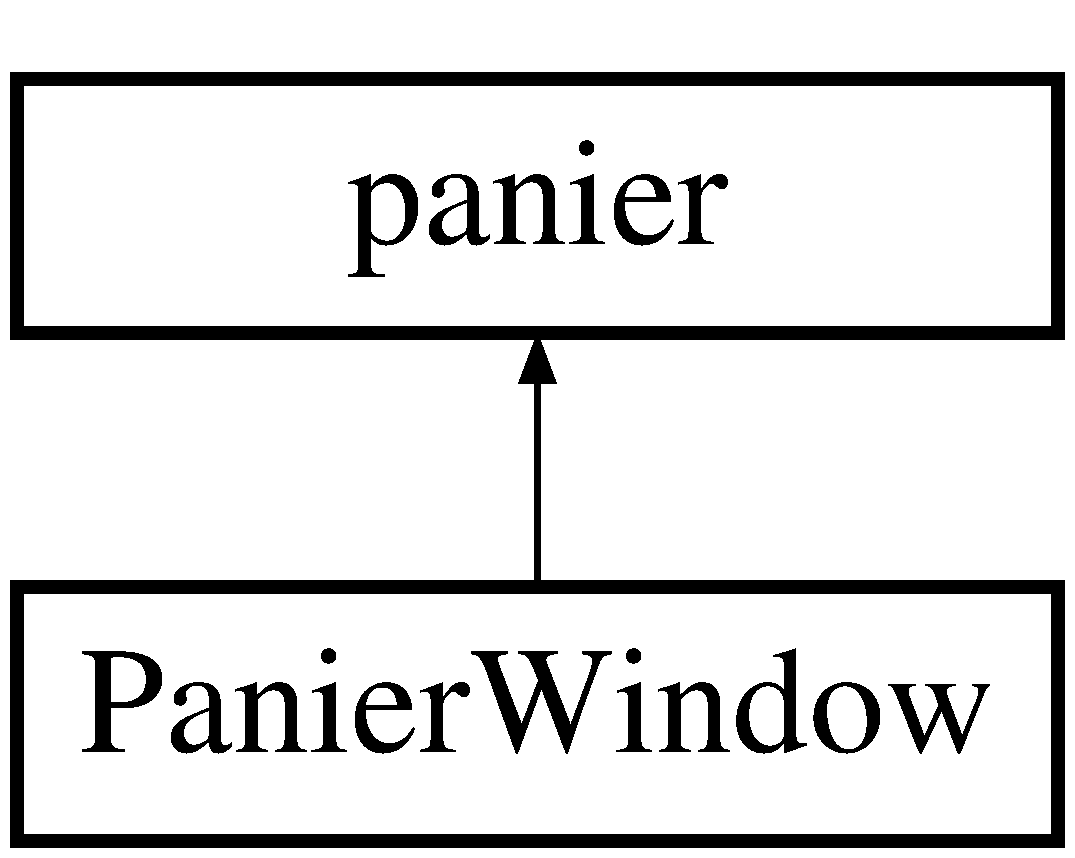
\includegraphics[height=2.000000cm]{classpanier}
\end{center}
\end{figure}
\subsection*{Public Member Functions}
\begin{DoxyCompactItemize}
\item 
{\bfseries panier} (vector$<$ \hyperlink{classplat}{plat} $\ast$ $>$ \+\_\+list\+Plat=\{\}, int \+\_\+num\+Client=0, int \+\_\+somme=0, int \+\_\+num\+Table=0)\hypertarget{classpanier_ac95e53b14831508e576d6fe9ea6ca4d0}{}\label{classpanier_ac95e53b14831508e576d6fe9ea6ca4d0}

\item 
vector$<$ \hyperlink{classplat}{plat} $\ast$ $>$ {\bfseries get\+List\+Plat} () const \hypertarget{classpanier_a76c516370e2deea1b99cd61693e098d2}{}\label{classpanier_a76c516370e2deea1b99cd61693e098d2}

\item 
void {\bfseries set\+List\+Plat} (const vector$<$ \hyperlink{classplat}{plat} $\ast$ $>$ \&value)\hypertarget{classpanier_a22148a0f1c97ccd16b91b5d5c6945dde}{}\label{classpanier_a22148a0f1c97ccd16b91b5d5c6945dde}

\item 
int {\bfseries get\+Num\+Table} () const \hypertarget{classpanier_a670beac1f516240ffecbd72ba832b24b}{}\label{classpanier_a670beac1f516240ffecbd72ba832b24b}

\item 
void {\bfseries set\+Num\+Table} (int value)\hypertarget{classpanier_aa2359acb3f72648b3cccfdba0b3417cb}{}\label{classpanier_aa2359acb3f72648b3cccfdba0b3417cb}

\item 
int {\bfseries get\+Num\+Client} () const \hypertarget{classpanier_a33b13ebeab9d67cd47d4e8b824bc7804}{}\label{classpanier_a33b13ebeab9d67cd47d4e8b824bc7804}

\item 
void {\bfseries set\+Num\+Client} (int value)\hypertarget{classpanier_a21c30ce458e025d8e5928c3524d23c82}{}\label{classpanier_a21c30ce458e025d8e5928c3524d23c82}

\item 
int {\bfseries get\+Somme} () const \hypertarget{classpanier_a19af7f142c7c34154dd79f4d5e047b01}{}\label{classpanier_a19af7f142c7c34154dd79f4d5e047b01}

\item 
void {\bfseries set\+Somme} (int value)\hypertarget{classpanier_abab52c08e4aa915aab3401313beca893}{}\label{classpanier_abab52c08e4aa915aab3401313beca893}

\end{DoxyCompactItemize}
\subsection*{Protected Attributes}
\begin{DoxyCompactItemize}
\item 
vector$<$ \hyperlink{classplat}{plat} $\ast$ $>$ {\bfseries list\+Plat}\hypertarget{classpanier_ad59ee07eb95540ab91ae06ac9738a831}{}\label{classpanier_ad59ee07eb95540ab91ae06ac9738a831}

\item 
int {\bfseries num\+Client}\hypertarget{classpanier_a791c7c33b74a67d1dd73c5adafaf8732}{}\label{classpanier_a791c7c33b74a67d1dd73c5adafaf8732}

\item 
int {\bfseries somme}\hypertarget{classpanier_acbe02df332222969cdebddfc573bad6d}{}\label{classpanier_acbe02df332222969cdebddfc573bad6d}

\item 
int {\bfseries num\+Table}\hypertarget{classpanier_a76dd23c4c09e2d1212d131ca255ee085}{}\label{classpanier_a76dd23c4c09e2d1212d131ca255ee085}

\end{DoxyCompactItemize}


The documentation for this class was generated from the following files\+:\begin{DoxyCompactItemize}
\item 
panier.\+h\item 
panier.\+cpp\end{DoxyCompactItemize}

\hypertarget{class_panier_window}{}\section{Panier\+Window Class Reference}
\label{class_panier_window}\index{Panier\+Window@{Panier\+Window}}
Inheritance diagram for Panier\+Window\+:\begin{figure}[H]
\begin{center}
\leavevmode
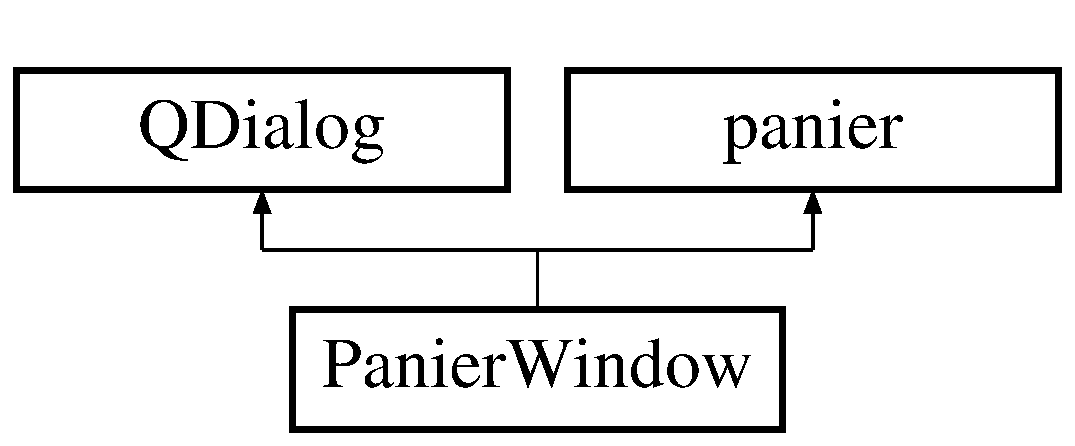
\includegraphics[height=2.000000cm]{class_panier_window}
\end{center}
\end{figure}
\subsection*{Public Slots}
\begin{DoxyCompactItemize}
\item 
void {\bfseries add\+Plat} (\hyperlink{classplat}{plat} $\ast$)\hypertarget{class_panier_window_ad010670d90a8c8bd5c1937dddc1517be}{}\label{class_panier_window_ad010670d90a8c8bd5c1937dddc1517be}

\item 
void {\bfseries delete\+Plat} (int idx)\hypertarget{class_panier_window_a9cad686a2a08a809a593ac58df259655}{}\label{class_panier_window_a9cad686a2a08a809a593ac58df259655}

\item 
void {\bfseries add\+Client} ()\hypertarget{class_panier_window_ad80148d8378357e609b8bfb1e7f92d08}{}\label{class_panier_window_ad80148d8378357e609b8bfb1e7f92d08}

\item 
void {\bfseries update\+Client} (bool)\hypertarget{class_panier_window_a8bcf2fe31a62a0ddc71a06dc32d5b54b}{}\label{class_panier_window_a8bcf2fe31a62a0ddc71a06dc32d5b54b}

\item 
void {\bfseries confirm\+Order} ()\hypertarget{class_panier_window_aacc7f49aa43eed49c85e340b184135ac}{}\label{class_panier_window_aacc7f49aa43eed49c85e340b184135ac}

\item 
void {\bfseries pay\+Bill} ()\hypertarget{class_panier_window_a8c2d6336d1d3bb4fb3041fb0e8c591e3}{}\label{class_panier_window_a8c2d6336d1d3bb4fb3041fb0e8c591e3}

\end{DoxyCompactItemize}
\subsection*{Signals}
\begin{DoxyCompactItemize}
\item 
void {\bfseries panier\+Updated} ()\hypertarget{class_panier_window_a059e18b2912d43ccdaba98943b699f8e}{}\label{class_panier_window_a059e18b2912d43ccdaba98943b699f8e}

\item 
void {\bfseries order\+Comfirmed} ()\hypertarget{class_panier_window_abf1be94aa02ed66ed7748433afc0d031}{}\label{class_panier_window_abf1be94aa02ed66ed7748433afc0d031}

\end{DoxyCompactItemize}
\subsection*{Public Member Functions}
\begin{DoxyCompactItemize}
\item 
{\bfseries Panier\+Window} (Q\+Widget $\ast$parent=0, vector$<$ \hyperlink{classplat}{plat} $\ast$ $>$ \+\_\+list\+Plat=\{\}, int \+\_\+num\+Client=0, int \+\_\+somme=0, int \+\_\+num\+Table=0)\hypertarget{class_panier_window_a03625b947e777b58c3dab33657d62753}{}\label{class_panier_window_a03625b947e777b58c3dab33657d62753}

\item 
void {\bfseries set\+Client} ()\hypertarget{class_panier_window_af41e891bf03a3decb1f37ddf7282d8d9}{}\label{class_panier_window_af41e891bf03a3decb1f37ddf7282d8d9}

\item 
int {\bfseries get\+Num\+Plat} () const \hypertarget{class_panier_window_a84e5101efc685171bcce0dcd7816a20e}{}\label{class_panier_window_a84e5101efc685171bcce0dcd7816a20e}

\item 
void {\bfseries set\+Static} ()\hypertarget{class_panier_window_a96b962be7668b710cf9a0dfe6682e9e7}{}\label{class_panier_window_a96b962be7668b710cf9a0dfe6682e9e7}

\item 
void {\bfseries clear} ()\hypertarget{class_panier_window_a058823a91b93f36c405480f21d4ef67b}{}\label{class_panier_window_a058823a91b93f36c405480f21d4ef67b}

\end{DoxyCompactItemize}
\subsection*{Additional Inherited Members}


The documentation for this class was generated from the following files\+:\begin{DoxyCompactItemize}
\item 
panierwindow.\+h\item 
panierwindow.\+cpp\end{DoxyCompactItemize}

\hypertarget{classplat}{}\section{plat Class Reference}
\label{classplat}\index{plat@{plat}}
Inheritance diagram for plat\+:\begin{figure}[H]
\begin{center}
\leavevmode
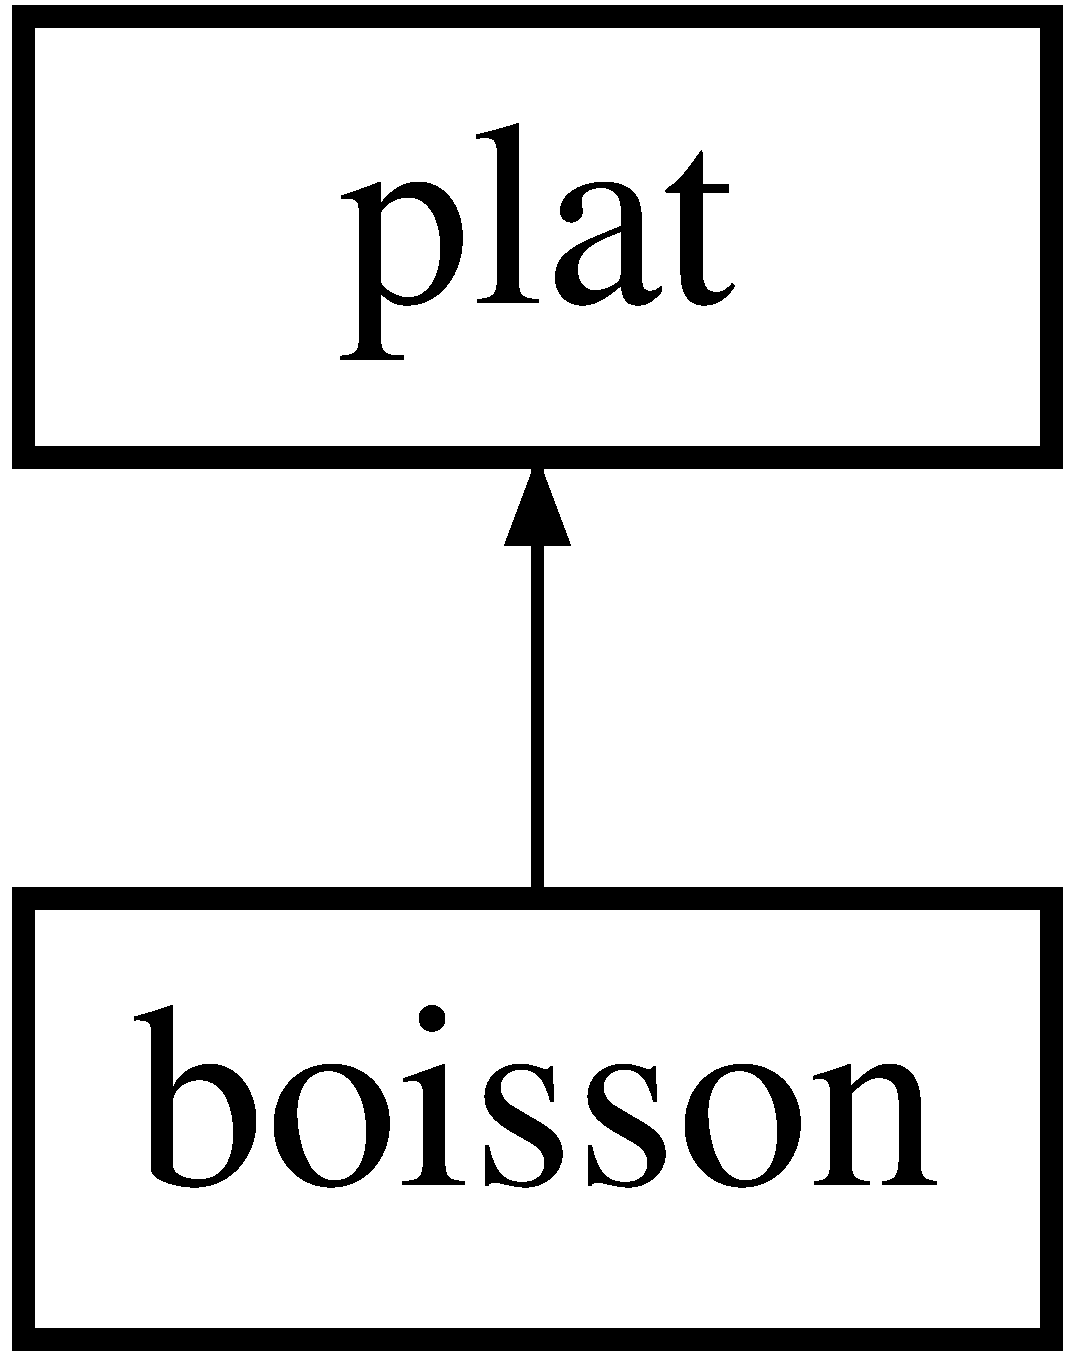
\includegraphics[height=2.000000cm]{classplat}
\end{center}
\end{figure}
\subsection*{Public Member Functions}
\begin{DoxyCompactItemize}
\item 
{\bfseries plat} (string \+\_\+nom, vector$<$ string $>$ \+\_\+ingredient=\{\}, int \+\_\+avis=-\/1, int \+\_\+calorie=-\/1, int \+\_\+prix=-\/1, const Q\+String image\+Path=\char`\"{}\+:my\+Images/image/testpic2.\+png\char`\"{})\hypertarget{classplat_a1d7b99afbf5d26ce34478012782265ee}{}\label{classplat_a1d7b99afbf5d26ce34478012782265ee}

\item 
string {\bfseries get\+Nom} () const \hypertarget{classplat_a172b4fa5c6bb8353e393205be28a2a3d}{}\label{classplat_a172b4fa5c6bb8353e393205be28a2a3d}

\item 
void {\bfseries set\+Nom} (const string \&value)\hypertarget{classplat_a28a571789cdb478907d31f572454bd4a}{}\label{classplat_a28a571789cdb478907d31f572454bd4a}

\item 
vector$<$ string $>$ {\bfseries get\+Ingredient} () const \hypertarget{classplat_aa86ce997d1672e9786d1a52647cf82a0}{}\label{classplat_aa86ce997d1672e9786d1a52647cf82a0}

\item 
void {\bfseries set\+Ingredient} (const vector$<$ string $>$ \&value)\hypertarget{classplat_a99fc4f43099e6e798541c7ad950afa27}{}\label{classplat_a99fc4f43099e6e798541c7ad950afa27}

\item 
int {\bfseries get\+Avis} () const \hypertarget{classplat_a95882ac8b6748992bc5657efa4059a20}{}\label{classplat_a95882ac8b6748992bc5657efa4059a20}

\item 
void {\bfseries set\+Avis} (int value)\hypertarget{classplat_a184976424abe4e9b8821b801bdac2e64}{}\label{classplat_a184976424abe4e9b8821b801bdac2e64}

\item 
int {\bfseries get\+Calorie} () const \hypertarget{classplat_a2bea33308a19317150126b8a5258afcb}{}\label{classplat_a2bea33308a19317150126b8a5258afcb}

\item 
void {\bfseries set\+Calorie} (int value)\hypertarget{classplat_a3950a6fa28af22b321046da35e507e5a}{}\label{classplat_a3950a6fa28af22b321046da35e507e5a}

\item 
int {\bfseries get\+Prix} () const \hypertarget{classplat_a012fa79385654ae6af325d3837b67e45}{}\label{classplat_a012fa79385654ae6af325d3837b67e45}

\item 
void {\bfseries set\+Prix} (int value)\hypertarget{classplat_a7e93c36df32773e7795b53ed1cf33858}{}\label{classplat_a7e93c36df32773e7795b53ed1cf33858}

\item 
Q\+Pixmap $\ast$ {\bfseries get\+Image} () const \hypertarget{classplat_a31232ed48766ff638057afc0ffe95ee2}{}\label{classplat_a31232ed48766ff638057afc0ffe95ee2}

\item 
void {\bfseries set\+Image} (const Q\+String value)\hypertarget{classplat_ac5862c8bf2fe8cad875246f32552af33}{}\label{classplat_ac5862c8bf2fe8cad875246f32552af33}

\item 
string {\bfseries get\+Description} () const \hypertarget{classplat_afc604b710f40dc9a883b2ee7744b5fdc}{}\label{classplat_afc604b710f40dc9a883b2ee7744b5fdc}

\item 
void {\bfseries set\+Description} (const string \&value)\hypertarget{classplat_a3e68a4e2b479609ea310210960beae6f}{}\label{classplat_a3e68a4e2b479609ea310210960beae6f}

\item 
void {\bfseries print\+Attrib} ()\hypertarget{classplat_a65ef0271840d18f29bf409b929a75b7f}{}\label{classplat_a65ef0271840d18f29bf409b929a75b7f}

\end{DoxyCompactItemize}
\subsection*{Protected Attributes}
\begin{DoxyCompactItemize}
\item 
string {\bfseries nom}\hypertarget{classplat_a3c797e85405202eeb72d27e9358bb48c}{}\label{classplat_a3c797e85405202eeb72d27e9358bb48c}

\item 
vector$<$ string $>$ {\bfseries ingredient}\hypertarget{classplat_aae512984318bde2cf4eeee899356d512}{}\label{classplat_aae512984318bde2cf4eeee899356d512}

\item 
int {\bfseries avis}\hypertarget{classplat_a8ff6d91450dda37738ca53b6cb12f5ce}{}\label{classplat_a8ff6d91450dda37738ca53b6cb12f5ce}

\item 
int {\bfseries calorie}\hypertarget{classplat_afc100e872d21ec0b2107649a76890113}{}\label{classplat_afc100e872d21ec0b2107649a76890113}

\item 
int {\bfseries prix}\hypertarget{classplat_aa1a30c5d06b80832f9d9bba4c42e49ae}{}\label{classplat_aa1a30c5d06b80832f9d9bba4c42e49ae}

\item 
Q\+Pixmap $\ast$ {\bfseries image}\hypertarget{classplat_ac9e759af7eec13f84be5da06428de68c}{}\label{classplat_ac9e759af7eec13f84be5da06428de68c}

\item 
string {\bfseries description}\hypertarget{classplat_acb4ed458ba6346de0b46fd3edb988a6b}{}\label{classplat_acb4ed458ba6346de0b46fd3edb988a6b}

\end{DoxyCompactItemize}


The documentation for this class was generated from the following files\+:\begin{DoxyCompactItemize}
\item 
plat.\+h\item 
plat.\+cpp\end{DoxyCompactItemize}

\hypertarget{classplat_intro}{}\section{plat\+Intro Class Reference}
\label{classplat_intro}\index{plat\+Intro@{plat\+Intro}}
Inheritance diagram for plat\+Intro\+:\begin{figure}[H]
\begin{center}
\leavevmode
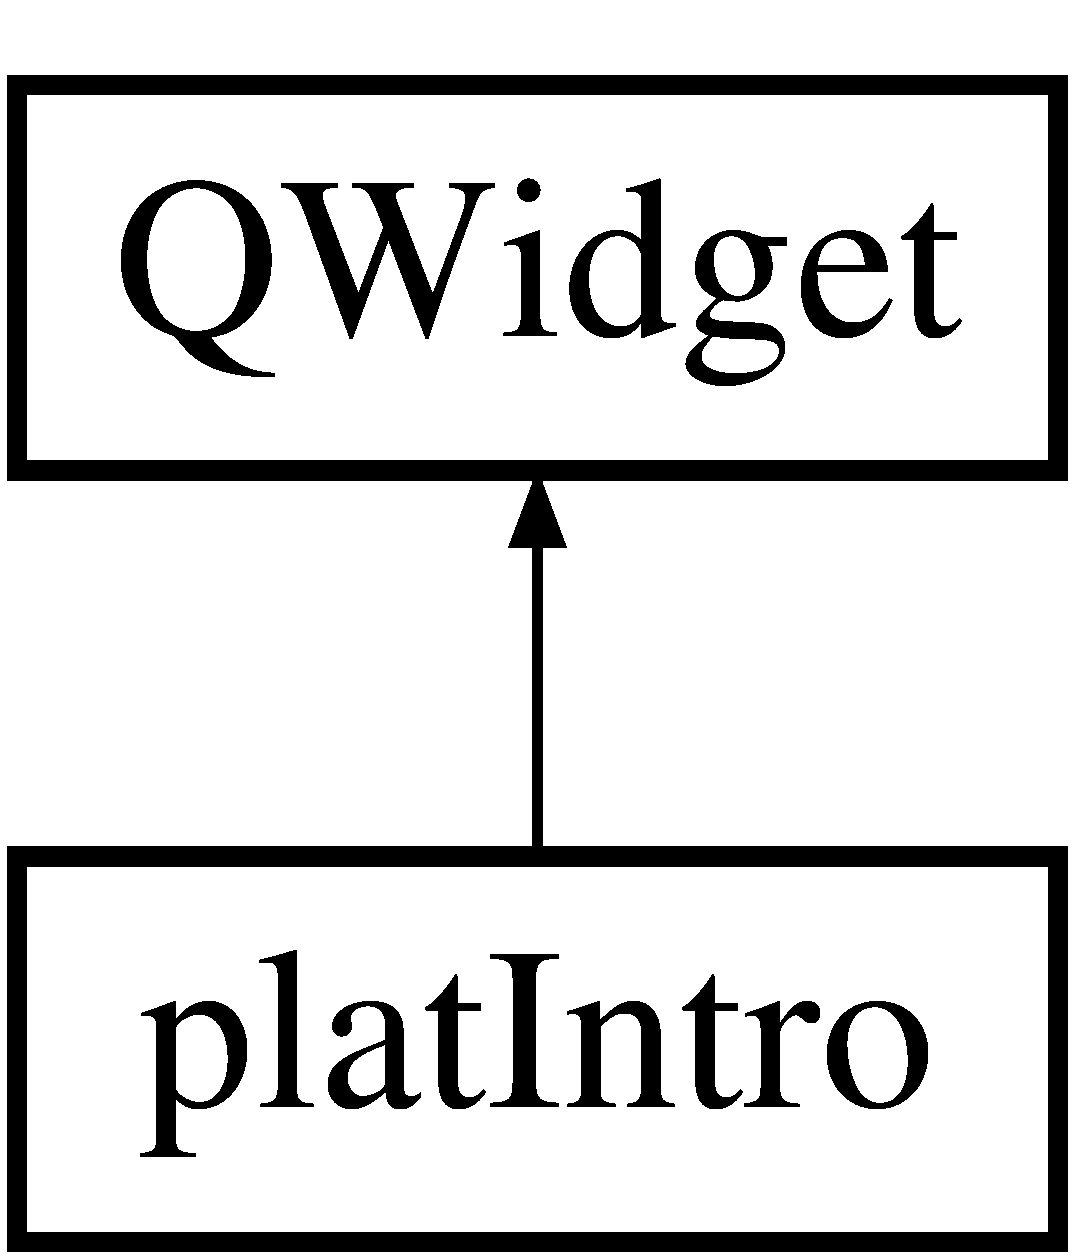
\includegraphics[height=2.000000cm]{classplat_intro}
\end{center}
\end{figure}
\subsection*{Signals}
\begin{DoxyCompactItemize}
\item 
void {\bfseries add\+To\+Panier} (\hyperlink{classplat}{plat} $\ast$)\hypertarget{classplat_intro_a644b0ffab5e616c74b4dc1f8c39456ce}{}\label{classplat_intro_a644b0ffab5e616c74b4dc1f8c39456ce}

\item 
void {\bfseries afficher\+Details} (\hyperlink{classplat}{plat} $\ast$)\hypertarget{classplat_intro_ad38a159413cf4f59d253fa33d5d230ff}{}\label{classplat_intro_ad38a159413cf4f59d253fa33d5d230ff}

\end{DoxyCompactItemize}
\subsection*{Public Member Functions}
\begin{DoxyCompactItemize}
\item 
{\bfseries plat\+Intro} (Q\+Widget $\ast$parent=0)\hypertarget{classplat_intro_a4db615d8dfa4a0ad020d88a36d954f27}{}\label{classplat_intro_a4db615d8dfa4a0ad020d88a36d954f27}

\item 
{\bfseries plat\+Intro} (\hyperlink{classplat}{plat} $\ast$\hyperlink{classplat}{plat})\hypertarget{classplat_intro_a4b5c0582a5ba0f0a22b2b2956c21285e}{}\label{classplat_intro_a4b5c0582a5ba0f0a22b2b2956c21285e}

\item 
void {\bfseries Set\+Up\+Layout} (\hyperlink{classplat}{plat} $\ast$\hyperlink{classplat}{plat})\hypertarget{classplat_intro_a075ae379eb15b767b3323f68b0d8f92c}{}\label{classplat_intro_a075ae379eb15b767b3323f68b0d8f92c}

\item 
virtual void {\bfseries paint\+Event} (Q\+Paint\+Event $\ast$)\hypertarget{classplat_intro_a3b164a28da5ee049e724a36c5256e684}{}\label{classplat_intro_a3b164a28da5ee049e724a36c5256e684}

\end{DoxyCompactItemize}
\subsection*{Public Attributes}
\begin{DoxyCompactItemize}
\item 
Q\+H\+Box\+Layout $\ast$ {\bfseries layout\+Global}\hypertarget{classplat_intro_a04721e0c108bec838bf50eb55d876b43}{}\label{classplat_intro_a04721e0c108bec838bf50eb55d876b43}

\item 
Q\+H\+Box\+Layout $\ast$ {\bfseries layout\+Image}\hypertarget{classplat_intro_ad37ba70bb06c3f8bf6ce6b5239f54084}{}\label{classplat_intro_ad37ba70bb06c3f8bf6ce6b5239f54084}

\item 
Q\+V\+Box\+Layout $\ast$ {\bfseries layout\+Descrip}\hypertarget{classplat_intro_ad1c42e7ee46cb3200108bdbee9aea852}{}\label{classplat_intro_ad1c42e7ee46cb3200108bdbee9aea852}

\item 
Q\+H\+Box\+Layout $\ast$ {\bfseries layout\+Plat\+Name}\hypertarget{classplat_intro_a6bfc90f5a1e536c1b0beaa697eec310b}{}\label{classplat_intro_a6bfc90f5a1e536c1b0beaa697eec310b}

\item 
Q\+H\+Box\+Layout $\ast$ {\bfseries layout\+Plat\+Etoile}\hypertarget{classplat_intro_a77a9a5fb503842c3af4c917e4b6b67c4}{}\label{classplat_intro_a77a9a5fb503842c3af4c917e4b6b67c4}

\item 
Q\+H\+Box\+Layout $\ast$ {\bfseries layout\+Show\+Detail}\hypertarget{classplat_intro_abcc680ffa3a0b5c0d87033bbc917f122}{}\label{classplat_intro_abcc680ffa3a0b5c0d87033bbc917f122}

\item 
Q\+Label $\ast$ {\bfseries show\+Image}\hypertarget{classplat_intro_a8a8337e79d98538a66a255fe9cbf2222}{}\label{classplat_intro_a8a8337e79d98538a66a255fe9cbf2222}

\item 
Q\+Push\+Button $\ast$ {\bfseries show\+Detail}\hypertarget{classplat_intro_ac24d01413affd6ad5cd24109d0b6b277}{}\label{classplat_intro_ac24d01413affd6ad5cd24109d0b6b277}

\item 
Q\+Push\+Button $\ast$ {\bfseries add}\hypertarget{classplat_intro_aa5672e30a23fa5d091883f2a2d868d31}{}\label{classplat_intro_aa5672e30a23fa5d091883f2a2d868d31}

\item 
Q\+Label $\ast$ {\bfseries show\+Name}\hypertarget{classplat_intro_a78548c02a78ec016f1c05dbf3d64aed5}{}\label{classplat_intro_a78548c02a78ec016f1c05dbf3d64aed5}

\item 
Q\+Label $\ast$ {\bfseries show\+Price}\hypertarget{classplat_intro_a37668428ca385c00f1fc498399427a17}{}\label{classplat_intro_a37668428ca385c00f1fc498399427a17}

\item 
Q\+Label $\ast$ {\bfseries show\+Avis}\hypertarget{classplat_intro_a30d5e086a48fa401d3d30cbda21e927f}{}\label{classplat_intro_a30d5e086a48fa401d3d30cbda21e927f}

\item 
\hyperlink{classplat}{plat} $\ast$ {\bfseries \+\_\+plat}\hypertarget{classplat_intro_a32bb65047ebeb69a2c9fe80d3fc87147}{}\label{classplat_intro_a32bb65047ebeb69a2c9fe80d3fc87147}

\end{DoxyCompactItemize}


The documentation for this class was generated from the following files\+:\begin{DoxyCompactItemize}
\item 
platintro.\+h\item 
platintro.\+cpp\end{DoxyCompactItemize}

%--- End generated contents ---

% Index
\backmatter
\newpage
\phantomsection
\clearemptydoublepage
\addcontentsline{toc}{chapter}{Index}
\printindex

\end{document}
